\documentclass[]{article}
\usepackage{lmodern}
\usepackage{amssymb,amsmath}
\usepackage{ifxetex,ifluatex}
\usepackage{fixltx2e} % provides \textsubscript
\ifnum 0\ifxetex 1\fi\ifluatex 1\fi=0 % if pdftex
  \usepackage[T1]{fontenc}
  \usepackage[utf8]{inputenc}
\else % if luatex or xelatex
  \ifxetex
    \usepackage{mathspec}
  \else
    \usepackage{fontspec}
  \fi
  \defaultfontfeatures{Ligatures=TeX,Scale=MatchLowercase}
\fi
% use upquote if available, for straight quotes in verbatim environments
\IfFileExists{upquote.sty}{\usepackage{upquote}}{}
% use microtype if available
\IfFileExists{microtype.sty}{%
\usepackage{microtype}
\UseMicrotypeSet[protrusion]{basicmath} % disable protrusion for tt fonts
}{}
\usepackage[margin=1in]{geometry}
\usepackage{hyperref}
\hypersetup{unicode=true,
            pdftitle={DATA 621 - Homework 1},
            pdfauthor={Joshua Sturm},
            pdfborder={0 0 0},
            breaklinks=true}
\urlstyle{same}  % don't use monospace font for urls
\usepackage{graphicx,grffile}
\makeatletter
\def\maxwidth{\ifdim\Gin@nat@width>\linewidth\linewidth\else\Gin@nat@width\fi}
\def\maxheight{\ifdim\Gin@nat@height>\textheight\textheight\else\Gin@nat@height\fi}
\makeatother
% Scale images if necessary, so that they will not overflow the page
% margins by default, and it is still possible to overwrite the defaults
% using explicit options in \includegraphics[width, height, ...]{}
\setkeys{Gin}{width=\maxwidth,height=\maxheight,keepaspectratio}
\usepackage[normalem]{ulem}
% avoid problems with \sout in headers with hyperref:
\pdfstringdefDisableCommands{\renewcommand{\sout}{}}
\IfFileExists{parskip.sty}{%
\usepackage{parskip}
}{% else
\setlength{\parindent}{0pt}
\setlength{\parskip}{6pt plus 2pt minus 1pt}
}
\setlength{\emergencystretch}{3em}  % prevent overfull lines
\providecommand{\tightlist}{%
  \setlength{\itemsep}{0pt}\setlength{\parskip}{0pt}}
\setcounter{secnumdepth}{0}
% Redefines (sub)paragraphs to behave more like sections
\ifx\paragraph\undefined\else
\let\oldparagraph\paragraph
\renewcommand{\paragraph}[1]{\oldparagraph{#1}\mbox{}}
\fi
\ifx\subparagraph\undefined\else
\let\oldsubparagraph\subparagraph
\renewcommand{\subparagraph}[1]{\oldsubparagraph{#1}\mbox{}}
\fi

%%% Use protect on footnotes to avoid problems with footnotes in titles
\let\rmarkdownfootnote\footnote%
\def\footnote{\protect\rmarkdownfootnote}

%%% Change title format to be more compact
\usepackage{titling}

% Create subtitle command for use in maketitle
\newcommand{\subtitle}[1]{
  \posttitle{
    \begin{center}\large#1\end{center}
    }
}

\setlength{\droptitle}{-2em}
  \title{DATA 621 - Homework 1}
  \pretitle{\vspace{\droptitle}\centering\huge}
  \posttitle{\par}
  \author{Joshua Sturm}
  \preauthor{\centering\large\emph}
  \postauthor{\par}
  \predate{\centering\large\emph}
  \postdate{\par}
  \date{February 26, 2018}

\usepackage{booktabs}
\usepackage{longtable}
\usepackage{array}
\usepackage{multirow}
\usepackage[table]{xcolor}
\usepackage{wrapfig}
\usepackage{float}
\usepackage{colortbl}
\usepackage{pdflscape}
\usepackage{tabu}
\usepackage{threeparttable}
\usepackage[normalem]{ulem}

\begin{document}
\maketitle

\section{Introduction}\label{introduction}

In this homework assignment, you will explore, analyze and model a data
set containing approximately 2200 records. Each record represents a
professional baseball team from the years 1871 to 2006 inclusive. Each
record has the performance of the team for the given year, with all of
the statistics adjusted to match the performance of a 162 game season.
Your objective is to build a multiple linear regression model on the
training data to predict the number of wins for the team.

\section{1. Data Exploration}\label{data-exploration}

\subsection{1.1 Load packages}\label{load-packages}

\subsection{1.2 Read in data}\label{read-in-data}

\subsection{1.2.1 Create data dictionary}\label{create-data-dictionary}

\begin{table}[H]
\centering\rowcolors{2}{gray!6}{white}

\resizebox{\linewidth}{!}{\begin{tabular}{lll}
\hiderowcolors
\toprule
Variable Name & Definition & Theoretical effect\\
\midrule
\showrowcolors
TARGET\_WINS & Number of wins & Outcome variable\\
TEAM\_BATTING\_H & Base hits by batters (1B, 2B, 3B, HR) & Positive impact on wins\\
TEAM\_BATTING\_2B & Doubles by batters (2B) & Positive impact on wins\\
TEAM\_BATTING\_3B & Triples by batters (3B) & Positive impact on wins\\
TEAM\_BATTING\_HR & Homeruns by batters (4B) & Positive impact on wins\\
\addlinespace
TEAM\_BATTING\_BB & Walks by batters & Positive impact on wins\\
TEAM\_BATTING\_SO & Strikeouts by batter & Negative impact on wins\\
TEAM\_BASERUN\_SB & Stolen bases & Positive impact on wins\\
TEAM\_BASERUN\_CS & Caught stealing & Negative impact on wins\\
TEAM\_BATTING\_HBP & Batters hit by pitch (free base) & Positive impact on wins\\
\addlinespace
TEAM\_PITCHING\_H & Hits allowed & Negative impact on wins\\
TEAM\_PITCHING\_HR & Homeruns allowed & Positive impact on wins\\
TEAM\_PITCHING\_BB & Walks allowed & Negative impact on wins\\
TEAM\_PITCHING\_SO & Strikeouts by pitchers & Positive impact on wins\\
TEAM\_FIELDING\_E & Errors & Negative impact on wins\\
TEAM\_FIELDING\_DP & Double plays & Positive impact on wins\\
\bottomrule
\end{tabular}}
\rowcolors{2}{white}{white}
\end{table}

\subsection{1.3 Basic variable
statistics}\label{basic-variable-statistics}

\begin{table}[H]
\centering\rowcolors{2}{gray!6}{white}

\resizebox{\linewidth}{!}{\begin{tabular}{lrrrrrrrrr}
\hiderowcolors
\toprule
  & n & mean & sd & median & min & max & skew & kurtosis & se\\
\midrule
\showrowcolors
INDEX & 2276 & 1268.46353 & 736.34904 & 1270.5 & 1 & 2535 & 0.0042149 & -1.2167564 & 15.4346788\\
TARGET\_WINS & 2276 & 80.79086 & 15.75215 & 82.0 & 0 & 146 & -0.3987232 & 1.0274757 & 0.3301823\\
BATTING\_H & 2276 & 1469.26977 & 144.59120 & 1454.0 & 891 & 2554 & 1.5713335 & 7.2785261 & 3.0307891\\
BATTING\_2B & 2276 & 241.24692 & 46.80141 & 238.0 & 69 & 458 & 0.2151018 & 0.0061609 & 0.9810087\\
BATTING\_3B & 2276 & 55.25000 & 27.93856 & 47.0 & 0 & 223 & 1.1094652 & 1.5032418 & 0.5856226\\
\addlinespace
BATTING\_HR & 2276 & 99.61204 & 60.54687 & 102.0 & 0 & 264 & 0.1860421 & -0.9631189 & 1.2691285\\
BATTING\_BB & 2276 & 501.55888 & 122.67086 & 512.0 & 0 & 878 & -1.0257599 & 2.1828544 & 2.5713150\\
BATTING\_SO & 2174 & 735.60534 & 248.52642 & 750.0 & 0 & 1399 & -0.2978001 & -0.3207992 & 5.3301912\\
BASERUN\_SB & 2145 & 124.76177 & 87.79117 & 101.0 & 0 & 697 & 1.9724140 & 5.4896754 & 1.8955584\\
BASERUN\_CS & 1504 & 52.80386 & 22.95634 & 49.0 & 0 & 201 & 1.9762180 & 7.6203818 & 0.5919414\\
\addlinespace
BATTING\_HBP & 191 & 59.35602 & 12.96712 & 58.0 & 29 & 95 & 0.3185754 & -0.1119828 & 0.9382681\\
PITCHING\_H & 2276 & 1779.21046 & 1406.84293 & 1518.0 & 1137 & 30132 & 10.3295111 & 141.8396985 & 29.4889618\\
PITCHING\_HR & 2276 & 105.69859 & 61.29875 & 107.0 & 0 & 343 & 0.2877877 & -0.6046311 & 1.2848886\\
PITCHING\_BB & 2276 & 553.00791 & 166.35736 & 536.5 & 0 & 3645 & 6.7438995 & 96.9676398 & 3.4870317\\
PITCHING\_SO & 2174 & 817.73045 & 553.08503 & 813.5 & 0 & 19278 & 22.1745535 & 671.1891292 & 11.8621151\\
\addlinespace
FIELDING\_E & 2276 & 246.48067 & 227.77097 & 159.0 & 65 & 1898 & 2.9904656 & 10.9702717 & 4.7743279\\
FIELDING\_DP & 1990 & 146.38794 & 26.22639 & 149.0 & 52 & 228 & -0.3889390 & 0.1817397 & 0.5879114\\
\bottomrule
\end{tabular}}
\rowcolors{2}{white}{white}
\end{table}

The training data has 2276 cases, with 17 variables.

INDEX, as its name suggest, is simply an index, which we can remove.

TARGET\_WINS is our response variable, leaving the remaining 15
variables as our predictors.

Right off the bat \texttt{:)}, we notice the data has some oddities.
Some variables are relatively sparse, particularly BASERUN\_CS and
BATTING\_HBP. The latter two have so many missing cases, 772 (34\%) and
2085 (92\%) respectively, that it would be unreasonable to include them
for use in any meaningful statistical model, so they will require
further examining in part 3.

\subsection{1.4 Summary Graphs}\label{summary-graphs}

\subsubsection{1.4.1 Boxplot}\label{boxplot}

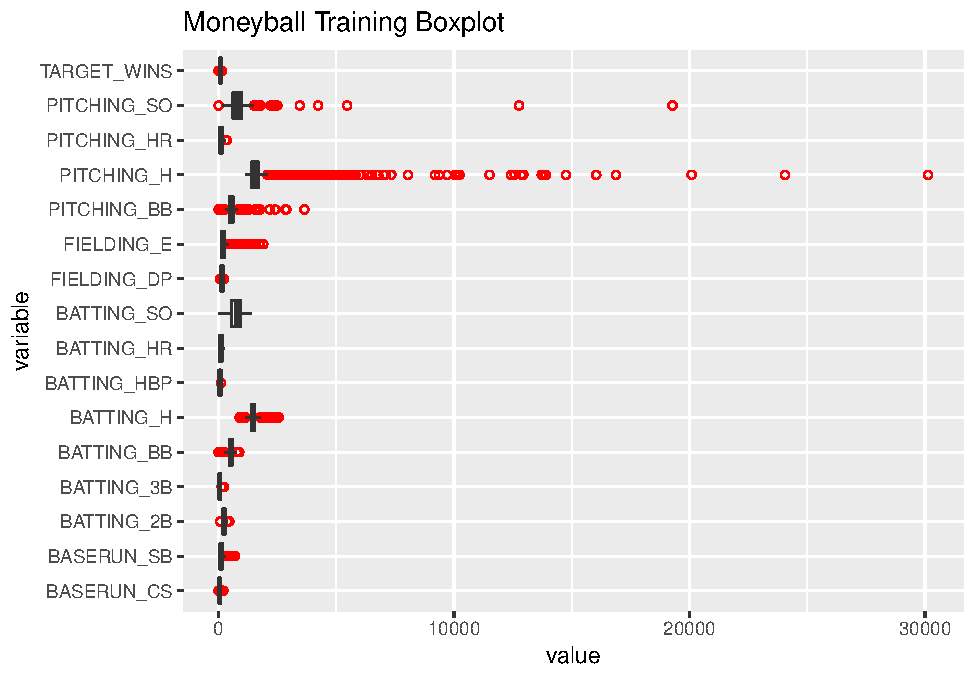
\includegraphics{DATA_621_Homework_1_files/figure-latex/summary-graph-boxplot-1.pdf}

\subsubsection{1.4.2 Histogram}\label{histogram}

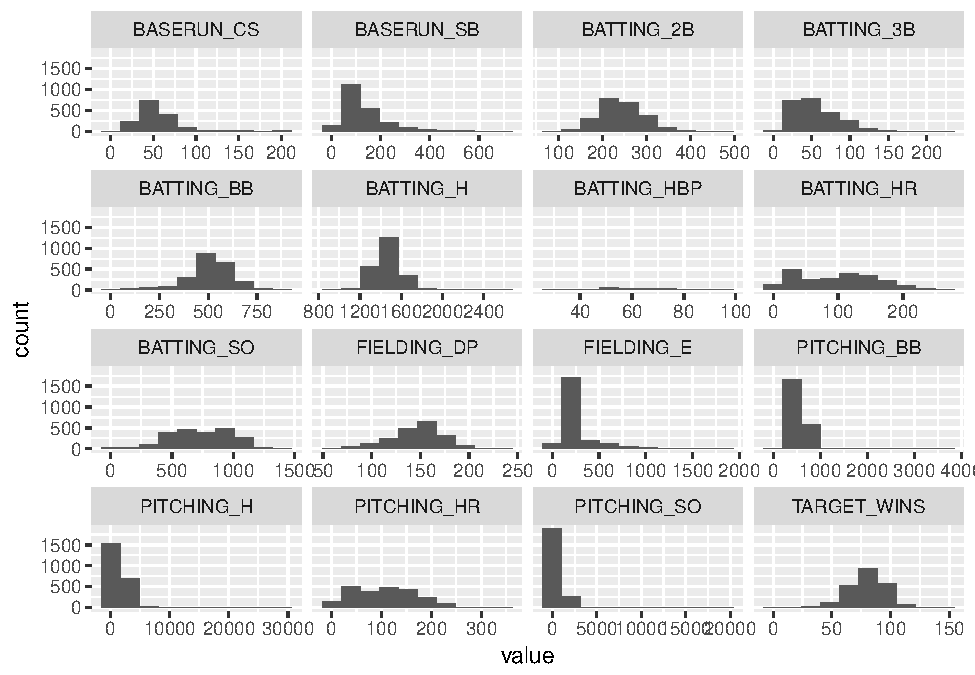
\includegraphics{DATA_621_Homework_1_files/figure-latex/summar-graph-hist-1.pdf}

\subsubsection{1.5 Correlation}\label{correlation}

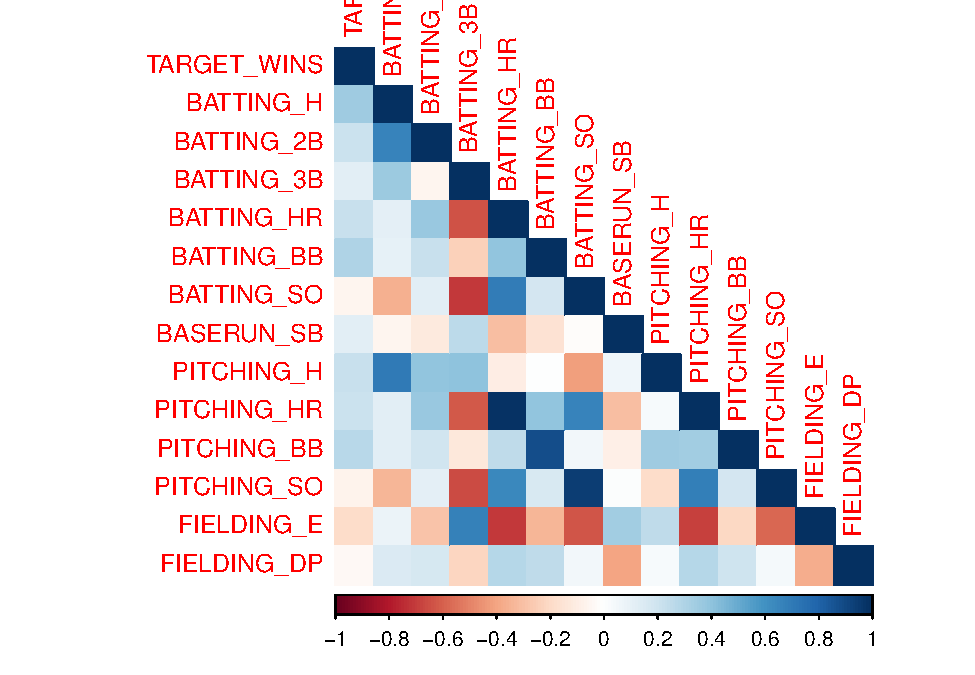
\includegraphics{DATA_621_Homework_1_files/figure-latex/summary-correlation-1.pdf}

\section{2. Data Preparation}\label{data-preparation}

\subsection{2.1 Adding and removing
variables}\label{adding-and-removing-variables}

From the above graphs, we notice a few things. Firstly, our response
variable, INDEX, is approximately normal.

Many of the predicting variables, however, are far from normal. I'll
address this in a few ways. Firstly, as can be seen in the data
dictionary, there are entries for \texttt{doubles}, \texttt{triples},
\texttt{homeruns}, and an all-encompassing \texttt{base\ hits}. Notably
missing is a variable for singles. I can create my own by simply taking
the difference between \texttt{base\ hits} and all three present
variables, i.e. \texttt{singles\ =} \texttt{base\ hits} -
\texttt{doubles} - \texttt{triples} - \texttt{homeruns}. Once I've
created my \texttt{singles} variable, I'll need to remove
\texttt{base\ hits} from the model to prevent multicollinearity.

Another issue is the strong correlation between \texttt{PITCHING\_HR}
and \texttt{BATTING\_HR} (97\%!), which makes sense - they're
essentially the same thing from opposite viewpoints. Since these
variables are practically the same as each other, we can safely drop one
of them.

As we mentioned in part 1, we're removing the two variables with a
significant amount of missing data - \texttt{BATTING\_HBP} and
\texttt{BASERUN\_CS}.

Additionally, FIELDING\_DP is missing 12.5\% of its total cases, so we
will drop it. The remaining variables have less than 6\% cases missing,
so we'll attempt to model with those in place.

\subsection{2.2 Missing data imputation}\label{missing-data-imputation}

While we removed the variables that were missing a large portion of
data, we're still left with others that have NA values.

BATTING\_SO, BASERUN\_SB, and PITCHING\_SO have an average of
\textasciitilde{} 112 missing cases.

After reading up on dealing with missing data in linear regression, it
seems that imputation by means of regression is preferred over a basic
statistical method such as mean, for example. To handle this, I'll make
use of the \texttt{Hmisc} package.

\subsection{2.3 Outliers}\label{outliers}

I'll begin by printing out the range for each variable, to see see if I
can identify any outliers based on the variable's extremes.

\begin{table}[H]
\centering\rowcolors{2}{gray!6}{white}

\resizebox{\linewidth}{!}{\begin{tabular}{rrrrrrrrrrrr}
\hiderowcolors
\toprule
TARGET\_WINS & BATTING\_2B & BATTING\_3B & BATTING\_HR & BATTING\_BB & BASERUN\_SB & PITCHING\_H & PITCHING\_BB & PITCHING\_SO & FIELDING\_E & BATTING\_1B & BATTING\_SO\\
\midrule
\showrowcolors
0 & 69 & 0 & 0 & 0 & 0 & 1137 & 0 & 0 & 65 & 709 & 0\\
146 & 458 & 223 & 264 & 878 & 697 & 30132 & 3645 & 19278 & 1898 & 2112 & 1399\\
\bottomrule
\end{tabular}}
\rowcolors{2}{white}{white}
\end{table}

When reviewing this table, together with the plots generated in part 1,
one can instantly notice oddities in the data. Going in order, I'll
begin with \texttt{BASERUN\_SB}. The team with the most stolen bases in
a season was the 1887 St.~Louis Cardinals with 581. I'll remove the
\texttt{sum(mb3\$BASERUN\_SB\ \textgreater{}\ 581)} rows which are
greater than 581.

MLB statistics show the 1915 Philadelphia Athletics to have the most
walks in a season, with 827. That works out to \textasciitilde{}859 in a
full 162-game season. Interestingly, removing the outliers for this
variable actually makes the model \emph{less} accurate; nevertheless, in
the interest of staying consistent, I will discard any row with a value
greater than 859.

Next is \texttt{PITCHING\_H}. I couldn't find any data on most hits
allowed, but according to
\href{https://en.wikipedia.org/wiki/List_of_Major_League_Baseball_hit_records}{this
list on wikipedia}, the most hits by a team in a season was 1,783, by
the Phillies in 1930. This raises questions about the original dataset's
max of \texttt{BATTING\_H} of 2,554. If a team allowed 30,132 hits in a
single season, that's an average of 186 hits per game\ldots{}which is
impossible. The record of 1,783 comes out to 11 hits per game. If they
played a full 162-game season, it would come out to 1,874.

Since such a large portion of this variable is in outlier territory, it
leads me to believe that it would be a mistake to discard the whole
thing. However, I'm not exactly sure how to deal with it; statistical
transformations, such as square root or log, have done little to rectify
the issue. I will resort to removing the 320 rows with values larger
than 1,874.

The next variable of concern is \texttt{PITCHING\_SO}. According to
official statistics kept by MLB (mlb.com), the team with the most
(pitching) strikeouts in a season was the 2017 Cleveland Indians, with a
staggering total of 1,614 strikeouts. Our data, however, has a max of
19278, which is several orders of magnitude larger than reality. So I
will remove the 12 rows larger than 1,614.

The third variable of concern is \texttt{FIELDING\_E}. The team with the
most fielding errors in a season was the \sout{1886 Washington
Nationals, with a total of 867} 1883 Baltimore Orioles, with 517. Since
there were only 98 games played then, that works out to
\textasciitilde{}854 in a full 162-game season. Thus, I will remove any
row with more errors than 854. This is also an interesting variable, in
that removing the outliers lowers the model's accuracy.

\section{3. Build models}\label{build-models}

\subsection{3.1 Model 1}\label{model-1}

I guess it makes the most sense to begin with a full model with all
(non-transformed) variables included.

\begin{verbatim}
## 
## Call:
## lm(formula = TARGET_WINS ~ ., data = mb.tr)
## 
## Residuals:
##      Min       1Q   Median       3Q      Max 
## -20.0626  -5.4196  -0.0423   5.2111  22.9355 
## 
## Coefficients:
##               Estimate Std. Error t value Pr(>|t|)    
## (Intercept) 60.4562317 19.7385030   3.063  0.00254 ** 
## INDEX       -0.0002478  0.0008508  -0.291  0.77122    
## BATTING_H    1.8111103  2.7908648   0.649  0.51723    
## BATTING_2B   0.0267462  0.0303941   0.880  0.38008    
## BATTING_3B  -0.1018043  0.0777401  -1.310  0.19208    
## BATTING_HR  -4.6100155 10.5666083  -0.436  0.66317    
## BATTING_BB  -4.4606275  3.6457882  -1.224  0.22279    
## BATTING_SO   0.4303282  2.6231874   0.164  0.86988    
## BASERUN_SB   0.0335937  0.0288100   1.166  0.24519    
## BASERUN_CS  -0.0130338  0.0719436  -0.181  0.85645    
## BATTING_HBP  0.0837038  0.0499097   1.677  0.09532 .  
## PITCHING_H  -1.7887761  2.7903398  -0.641  0.52233    
## PITCHING_HR  4.6958245 10.5649821   0.444  0.65725    
## PITCHING_BB  4.5120283  3.6432611   1.238  0.21721    
## PITCHING_SO -0.4618971  2.6214432  -0.176  0.86034    
## FIELDING_E  -0.1724513  0.0415365  -4.152 5.16e-05 ***
## FIELDING_DP -0.1063200  0.0371964  -2.858  0.00478 ** 
## ---
## Signif. codes:  0 '***' 0.001 '**' 0.01 '*' 0.05 '.' 0.1 ' ' 1
## 
## Residual standard error: 8.489 on 174 degrees of freedom
##   (2085 observations deleted due to missingness)
## Multiple R-squared:  0.5503, Adjusted R-squared:  0.509 
## F-statistic: 13.31 on 16 and 174 DF,  p-value: < 2.2e-16
\end{verbatim}

Not a very robust model; many insignificant variables, a low \(R^2\)
value, and a high AIC and BIC. There are also a lot of weird
coefficients in this model. Triples, \emph{home runs}, walks, (pitching)
strikeouts, and double plays all have negative coefficients, meaning
they are negatively correlated with the model.

\subsection{3.2 Model 2}\label{model-2}

The second model I'll try contains the dataset with the added and
removed variables, but none of them were transformed.

\begin{verbatim}
## 
## Call:
## lm(formula = TARGET_WINS ~ ., data = mb2)
## 
## Residuals:
##     Min      1Q  Median      3Q     Max 
## -44.840  -7.961   0.168   7.573  50.911 
## 
## Coefficients:
##               Estimate Std. Error t value Pr(>|t|)    
## (Intercept) 17.7010995  5.1280679   3.452 0.000568 ***
## BATTING_2B  -0.0081692  0.0071957  -1.135 0.256385    
## BATTING_3B   0.1205824  0.0165717   7.276 4.87e-13 ***
## BATTING_HR   0.1201699  0.0083181  14.447  < 2e-16 ***
## BATTING_BB   0.0255959  0.0064707   3.956 7.90e-05 ***
## BATTING_SO  -0.0081180  0.0050803  -1.598 0.110213    
## BASERUN_SB   0.0585237  0.0042963  13.622  < 2e-16 ***
## PITCHING_H   0.0024770  0.0004047   6.120 1.12e-09 ***
## PITCHING_BB -0.0027189  0.0051155  -0.531 0.595139    
## PITCHING_SO -0.0040271  0.0044839  -0.898 0.369221    
## FIELDING_E  -0.0499358  0.0032267 -15.476  < 2e-16 ***
## BATTING_1B   0.0396067  0.0037802  10.477  < 2e-16 ***
## ---
## Signif. codes:  0 '***' 0.001 '**' 0.01 '*' 0.05 '.' 0.1 ' ' 1
## 
## Residual standard error: 11.63 on 2031 degrees of freedom
##   (233 observations deleted due to missingness)
## Multiple R-squared:  0.3611, Adjusted R-squared:  0.3577 
## F-statistic: 104.4 on 11 and 2031 DF,  p-value: < 2.2e-16
\end{verbatim}

This model has more sensible coefficients, even though it scored lower
(\(R^2\)).

\subsection{3.3 Model 3}\label{model-3}

The third model will be the modified dataset with all the transformed
variables.

\begin{verbatim}
## 
## Call:
## lm(formula = TARGET_WINS ~ ., data = mb3)
## 
## Residuals:
##     Min      1Q  Median      3Q     Max 
## -37.163  -7.661   0.146   7.627  38.457 
## 
## Coefficients:
##              Estimate Std. Error t value Pr(>|t|)    
## (Intercept) 30.746279   5.765368   5.333 1.08e-07 ***
## BATTING_2B  -0.080753   0.019091  -4.230 2.45e-05 ***
## BATTING_3B   0.148211   0.024128   6.143 9.82e-10 ***
## BATTING_HR   0.045947   0.019711   2.331 0.019853 *  
## BATTING_BB   0.204607   0.050556   4.047 5.39e-05 ***
## BASERUN_SB   0.089149   0.004888  18.240  < 2e-16 ***
## PITCHING_H   0.060620   0.016882   3.591 0.000338 ***
## PITCHING_BB -0.165753   0.047778  -3.469 0.000533 ***
## PITCHING_SO  0.015239   0.008604   1.771 0.076693 .  
## FIELDING_E  -0.087109   0.004906 -17.757  < 2e-16 ***
## BATTING_1B  -0.033850   0.018148  -1.865 0.062293 .  
## BATTING_SO  -0.028905   0.008846  -3.267 0.001104 ** 
## ---
## Signif. codes:  0 '***' 0.001 '**' 0.01 '*' 0.05 '.' 0.1 ' ' 1
## 
## Residual standard error: 11.08 on 1940 degrees of freedom
## Multiple R-squared:  0.3794, Adjusted R-squared:  0.3759 
## F-statistic: 107.8 on 11 and 1940 DF,  p-value: < 2.2e-16
\end{verbatim}

The transformed model further improves on the second, with respect to
the coefficients. \texttt{PITCHING\_H} is positive instead of negative,
while \texttt{BATTING\_1B} and \texttt{BATTING\_2B} are negative.

\section{4. Model selection}\label{model-selection}

To ensure uniformity between the datasets, I performed the same
transformations on the evaluation set.

Here is a sample of the model's results:

\begin{table}[H]
\centering\rowcolors{2}{gray!6}{white}

\resizebox{\linewidth}{!}{\begin{tabular}{rrrl}
\hiderowcolors
\toprule
actuals & predicted & error & percerror\\
\midrule
\showrowcolors
70 & 63.70946 & -6.290544 & -8.99\%\\
86 & 69.05946 & -16.940545 & -19.7\%\\
70 & 72.50420 & 2.504199 & 3.58\%\\
82 & 84.20480 & 2.204797 & 2.69\%\\
75 & 76.53630 & 1.536295 & 2.05\%\\
80 & 70.07014 & -9.929861 & -12.41\%\\
\bottomrule
\end{tabular}}
\rowcolors{2}{white}{white}
\end{table}

\begin{verbatim}
## [1] "The mean error is: 1.78783769655456"
\end{verbatim}

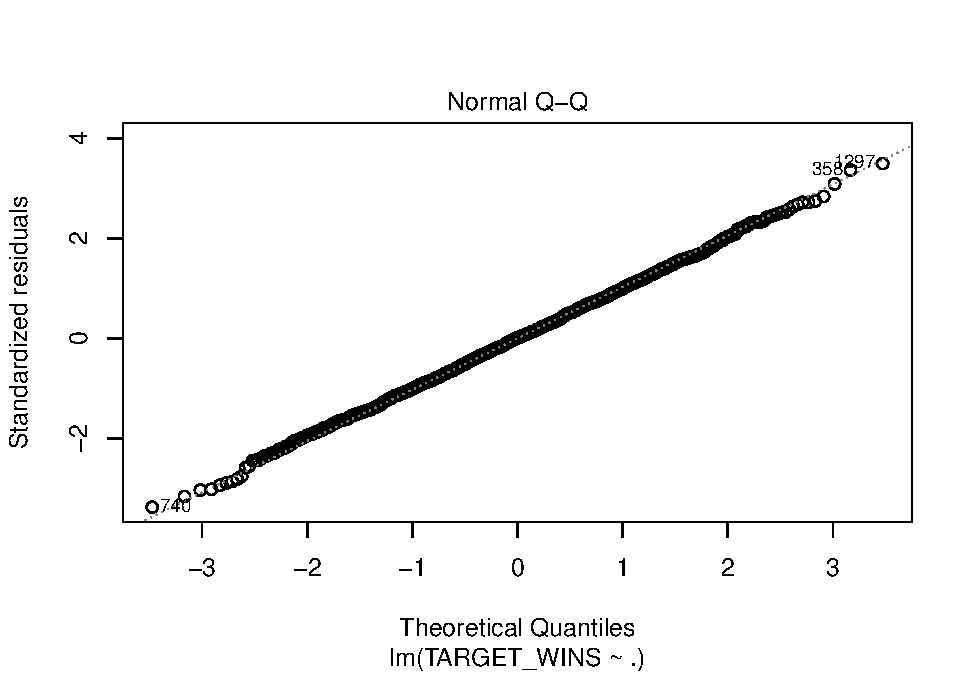
\includegraphics{DATA_621_Homework_1_files/figure-latex/predict-plots-1.pdf}
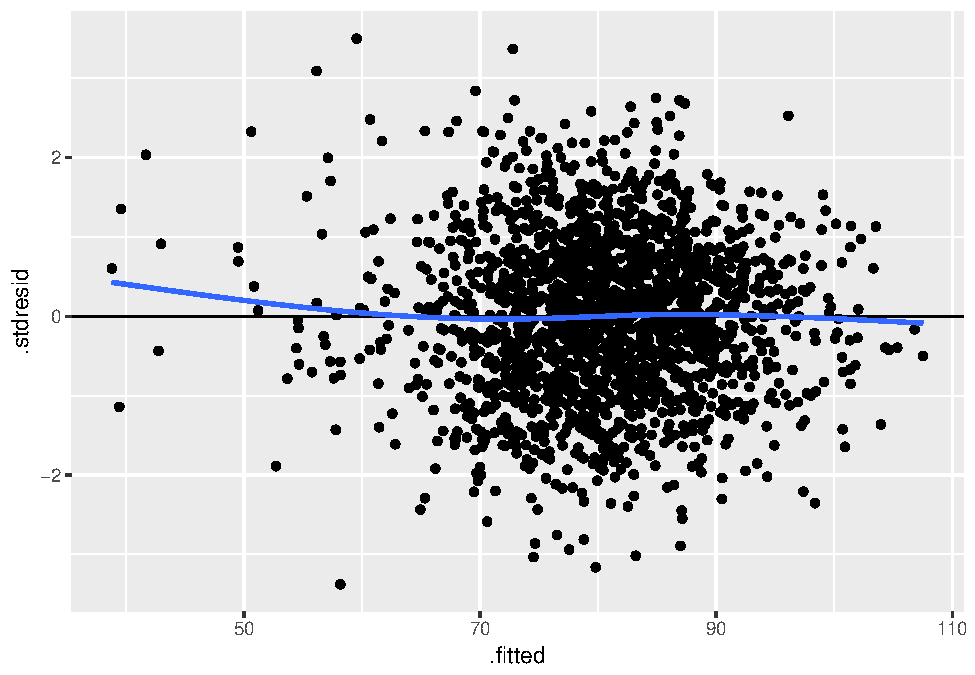
\includegraphics{DATA_621_Homework_1_files/figure-latex/predict-plots-2.pdf}
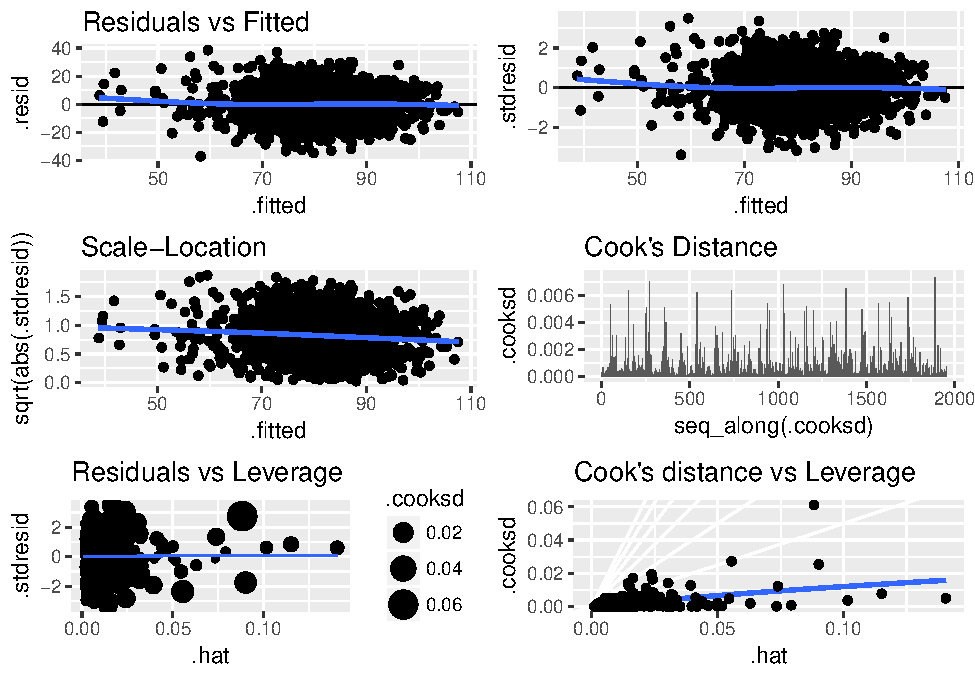
\includegraphics{DATA_621_Homework_1_files/figure-latex/predict-plots-3.pdf}

\section{5. Closing words}\label{closing-words}

I picked the third model, because I felt the data was the most honest -
that is, it had the fewest outliers, and was closer to what it was meant
to represent. The full model had a higher \(R^2\), but that could be
attributed to collinearity amongst the variables. The model is not
perfect, and I likely would not use it in practice, but, given the many
issues with the data, I believe I optimized it as best I could.

\section{References}\label{references}

\begin{itemize}
\tightlist
\item
  \url{https://www.analyticsvidhya.com/blog/2016/03/tutorial-powerful-packages-imputing-missing-values/}
\item
  \url{https://www.baseball-reference.com}
\item
  \url{https://www.baseball-almanac.com}
\item
  \url{https://www.mlb.com}
\item
  \url{https://sports.stackexchange.com/questions/16246/what-is-the-mlb-record-for-most-errors-by-one-team-in-one-season-during-the-mode}
\item
  \url{http://r-statistics.co/Linear-Regression.html}
\item
  \url{http://ggplot2.tidyverse.org/reference/fortify.lm.html}
\end{itemize}


\end{document}
